% %%%%%%%%%%%%%%%%%%%%%%%%%%%%%%%%%%%%%%%%%%%%%%%%%%%%%%%%%%%%%%%%%%%%%%%%

% %%% LaTeX Template for AAMAS-2026 (based on sample-sigconf.tex)
% %%% Prepared by the AAMAS-2026 Publication Chairs based on the version from AAMAS-2025. 

% %%%%%%%%%%%%%%%%%%%%%%%%%%%%%%%%%%%%%%%%%%%%%%%%%%%%%%%%%%%%%%%%%%%%%%%%

% %%% Start your document with the \documentclass command.


% %%% == IMPORTANT ==
% %%% Use the first variant below for the final paper (including author information).
% %%% Use the second variant below to anonymize your submission (no author information shown).
% %%% For further information on anonymity and double-blind reviewing, 
% %%% please consult the call for paper information
% %%% https://cyprusconferences.org/aamas2026/submission-instructions/

% %%%% For anonymized submission, use this
% \documentclass[sigconf,anonymous]{aamas} 

% %%%% For camera-ready, use this
% % \documentclass[sigconf]{aamas} 


% %%% Load required packages here (note that many are included already).

% \usepackage{balance} % for balancing columns on the final page


% % JE ADDED PACKAGES
% \usepackage{algorithm}
% \usepackage{algorithmic}
% \usepackage{booktabs}
% \usepackage{multirow}
% \usepackage{colortbl}
% \usepackage{xcolor}
% \usepackage[section]{placeins}
% \usepackage{amsmath,amssymb}
% \DeclareMathOperator*{\argmax}{arg\,max}
% \DeclareMathOperator*{\argmin}{arg\,min}
% \usepackage{caption}
% \usepackage{subcaption}
% \usepackage{todonotes}
% \usepackage{orcidlink}
% \usepackage{hyperref}
% \usepackage{stfloats}

% % Define colors
% \definecolor{fastest}{RGB}{0, 150, 100}   % Green for efficiency
% \definecolor{globalbest}{RGB}{0, 0, 200}  % Blue for absolute best 


% %%%%%%%%%%%%%%%%%%%%%%%%%%%%%%%%%%%%%%%%%%%%%%%%%%%%%%%%%%%%%%%%%%%%%%%%

% %%% AAMAS-2026 copyright block (do not change!)


% \setcopyright{none}
%     \acmConference[ALA '26]%
%     {Proc.\@ of the Adaptive and Learning Agents Workshop (ALA 2026)}%
%     {May 25 -- 26, 2026}%
%     {Paphos, Cyprus, https://alaworkshop2026.github.io/}%
%     {Aydeniz, Delgrange, Mohammedalamen, Yang (eds.)}%
%     \copyrightyear{2026}
%     \acmYear{2026}
%     \acmDOI{}
%     \acmPrice{}
%     \acmISBN{}
%     \settopmatter{printacmref=false}

% %%%%%%%%%%%%%%%%%%%%%%%%%%%%%%%%%%%%%%%%%%%%%%%%%%%%%%%%%%%%%%%%%%%%%%%%

% %%% == IMPORTANT ==
% %%% Use this command to specify your submission number.
% %%% In anonymous mode, it will be printed on the first page.

% \acmSubmissionID{<<submission id>>}

% %%% Use this command to specify the title of your paper.

% \title[Learning from coutnerfactuals]{Counterfactual Gradient Alignment: Optimizing Directional Expert Supervision for Data-Efficient Learning}

% %%% Provide names, affiliations, and email addresses for all authors.

% \author{Arthur Pendragon}
% \affiliation{
%   \institution{Camelot Castle}
%   \city{Camelot}
%   \country{United Kingdom}}
% \email{king.arthur@camelot.uk}

% \author{Nimue}
% \affiliation{
%   \institution{The Lady's Lake}
%   \city{Avalon}
%   \country{United Kingdom}}
% \email{lady.of.the.lake@avalon.uk}

% %%% Use this environment to specify a short abstract for your paper.





%%% Use this command to specify a few keywords describing your work.
%%% Keywords should be separated by commas.



% %%%%%%%%%%%%%%%%%%%%%%%%%%%%%%%%%%%%%%%%%%%%%%%%%%%%%%%%%%%%%%%%%%%%%%%%

% %%% Include any author-defined commands here.
         
% \newcommand{\BibTeX}{\rm B\kern-.05em{\sc i\kern-.025em b}\kern-.08em\TeX}

% %%%%%%%%%%%%%%%%%%%%%%%%%%%%%%%%%%%%%%%%%%%%%%%%%%%%%%%%%%%%%%%%%%%%%%%%

% \begin{document}

% %%% The following commands remove the headers in your paper. For final 
% %%% papers, these will be inserted during the pagination process.

% \pagestyle{fancy}
% \fancyhead{}

% %%% The next command prints the information defined in the preamble.

% \maketitle 

% %%%%%%%%%%%%%%%%%%%%%%%%%%%%%%%%%%%%%%%%%%%%%%%%%%%%%%%%%%%%%%%%%%%%%%%%
xmaker \chapter{Counterfactual Gradient Alignment: Optimizing Directional
Expert Supervision for Data-Efficient Learning}
\label{chap:learning_from_counterfactuals}


\begin{abstract}
Machine learning models typically require large amounts of labelled data and often fail to generalise to out-of-distribution examples. Humans, by contrast, apply prior knowledge and intuition to solve new problems rapidly, requiring far fewer examples. In this chapter we investigate how to address this disparity by enriching standard data-label pairs with gradient-based \emph{expert annotations}. We introduce the \textbf{Counterfactual Gradient Alignment (CGA)} framework, in which training examples are optionally augmented with a \emph{counterfactual direction}: a unit vector indicating the direction in feature space along which the model's predicted class should change. A family of directional loss functions penalises the model when its gradient is misaligned with these expert-provided directions, enforcing that class confidence decreases along counterfactual paths without requiring additional labelled data. We evaluate three loss variants---Sign, ReLU, and Softplus---across four synthetic 2D classification tasks and two natural language processing benchmarks (IMDB sentiment classification and AGNEWS topic classification) under varying degrees of data scarcity and with active-learning-based annotation selection. Our Softplus-Strong variant consistently accelerates learning and improves accuracy over standard cross-entropy baselines in most settings. We further present an interactive graphical interface enabling real-time counterfactual annotation by human experts~\cite{erskine2024ijcai}, and investigate entropy- and diversity-based importance sampling strategies to maximise the utility of a limited annotation budget.
\end{abstract}

\keywords{Counterfactuals, Supervised Learning, Human-in-the-loop, Gradient Supervision, Data Efficiency, Active Learning}

\section{Introduction}
Highly tailored machine learning models typically require large amounts of data and may fail to generalise well to out-of-distribution examples, leading to unexpected or inaccurate predictions \cite{hand_classifier, Challen231, souza2020challenges}. Humans are, by contrast, relatively fast learners. We are able to utilise information outside of the usual data-label pair that is provided to machine learning systems, requiring fewer data points in order to draw conclusions and generalise to unseen data. It would be trivial, for example, for a human to adapt from film reviews to political tweets when performing sentiment classification, where a machine learning (ML) model may require refinement \cite{blitzer-etal-2007-biographies}. When operating in real environments the underlying distribution of observable data is often dynamic, subject to change and has limited availability \cite{Sahiner2023}. Particularly when errors carry a high cost, be it monetary or a risk to human safety, strong generalisation is a necessary component of any model which aims to assist or replace a highly adaptable human supervisor.

Whether we must maximise the utility of a few available samples or adapt to new observations quickly, the objective is often to learn the underlying distribution from a minimal number of examples while avoiding over-fitting. In online settings such as Active Learning, lack of data is addressed by the machine learning algorithm communicating with a (typically human) oracle who returns a new label for each query example, usually selected to reduce a form of uncertainty~\cite{prince2004does}. Formulations like Machine Teaching approach the problem by allowing humans to select minimal groups of samples that effectively describe concepts and patterns \cite{Zhu2015}. Both approaches can be said to improve data efficiency and the ability of models to generalise to new data through an informed selection of training data.

In this chapter we describe an alternative approach: rather than querying an oracle for more labels, we enrich existing observations with \emph{complex annotations}. We propose that embedding additional information in the annotation and learning process can increase data efficiency, at the expense of annotation complexity. Specifically, we present one realisation of this idea by augmenting each training example with a \emph{counterfactual direction}---a unit vector indicating the direction in feature space along which the predicted class should change. We also propose a family of novel loss functions that enforce negative model gradients along these directions, with the intuition that a change in class should be reflected in the model's confidence surface. Where gradients have been used previously as a natural method for providing human-interpretable explanations~\cite{simonyan2013deep}, this chapter aims to reverse this pipeline and provide machine-interpretable supervision. To make this annotation scheme practical, we present a graphical user interface (GUI) that allows a human expert to observe the model's evolving decision surface and supply counterfactual direction annotations interactively during training, without requiring additional labelled examples; this interface was first introduced at IJCAI-24~\cite{erskine2024ijcai} and is described in Section~\ref{subsec:annotation_interface}.

Finally, we investigate entropy- and diversity-based importance sampling measures to maximise utility in highly data-limited regimes, strategically selecting the most informative samples for counterfactual annotation. This approach combines uncertainty-based selection (targeting samples where the model is most confused) with diversity constraints (ensuring broad coverage of the feature space), maximising the value of each human-provided annotation whilst avoiding redundant supervision in dense data regions.

The remainder of this chapter is organised as follows. Section~\ref{related_work} reviews related work on embedding human priors, learning from counterfactuals, and active learning. Section~\ref{sec:gradient_learning} introduces the CGA framework and interactive annotation interface. Section~\ref{sec:experimental_setup} describes the experimental setup, followed by results in Section~\ref{sec:results}, discussion in Section~\ref{sec:discussion}, and conclusions in Section~\ref{sec:conclusions}.

\section{Related Work}
\label{related_work}

% zero/few-shot learning
% objectives:
%         generalization
%         efficient adaptation
%         utilization of auxiliary information

% active learning
% To embed human priors in some form of annotation for use during training, we settle on the idea that counterfactuals provide a useful learning signal which can be passed from human to machine, and investigate how to generate counterfactuals and integrate this learning signal into the machine learning pipeline. Here we look at previous work which relates to each of these constituent components



In this section we review state-of-the-art methods for including additional information in machine learning systems that go beyond data-label pairs, namely; human priors, counterfactual observations and gradient supervision.

\subsection{Embedding human priors in model training}
One significant motivation of this work is to enable human annotators to provide domain knowledge to models to improve data efficiency. \citeauthor{rieger2020interpretations} \cite{rieger2020interpretations} demonstrated the ability to embed human priors in their work developing contextual decomposition explanation penalisation (CDEP). CDEP enables embedding domain knowledge during model training to ignore spurious correlations, correct errors, and generalise to different types of dataset shifts. This method assumes that the explanation method is truthful and penalises model explanations where these do not align with explanations provided by an oracle. Domain knowledge can be encoded by a human or in an automated fashion. In a similar fashion, Ross et al. embed human priors as explanations and develop a loss function which balances cross entropy loss with an additional function to penalise misaligned model explanations \cite{ross2017right}. In their applications, they reinforce the magnitude of gradients to align to pre-supposed explanation; penalising the model where features are inappropriately neglected or considered to be too important.

\subsection{Training with counterfactuals}
Kaushik et al. \cite{Kaushik2020Learning} present a system for collecting counterfactually augmented data by tasking human annotators to minimally edit individual observations to produce a counterfactual on a subset of the IMDB dataset \cite{imdb}. They demonstrate that incorporating counterfactuals within the training data leads to improved generalisation and show that training purely with unaltered data or counterfactual pairs leads to over-fitting on spurious signals, while a combined dataset produces a model which is less sensitive to these signals.

In a follow up paper, Kaushik et al. investigate why counterfactually augmented data reduces spurious correlations \cite{kaushik2021explaining}. They propose that adding noise over causal features should worsen in-domain and out-of-domain performance, but that adding noise to non-causal features should improve relative performance on out-of-domain tasks. To test this hypothesis, they apply noise to the complement of the edited sections of text within their counterfactually augmented dataset. They repeat this process for sections of text identified by an attention-based classifier (BiLSTM with Self-Attention \cite{graves2005framewise}) and by gradient-based feature attribution \cite{li2016visualizing}, and find that human annotations served as the best augmentation for performance on out-of-distribution data. 

In our work we evaluate models trained on the counterfactually augmented data produced both by humans and algorithmically. However, we take a different approach to learning from these counterfactual augmentations through gradient supervision.

\subsection{Learning from counterfactuals through gradient supervision}
\label{subsec:gradient_supervision}
Teney et al. \cite{teney2020learning} introduce a novel training objective called ``gradient supervision", which involves penalising the angle between the gradients of a neural network classifier and the vector difference between counterfactual examples in the input space. Using a counterfactual, Teney et al. define a loss function which aims to minimise the angle between the model gradient and vector pointing to the counterfactual as 
\begin{equation}
        \mathcal{L}_{GS} \left(\mathbf{g}_i,\hat{\mathbf{g}}_i \right)  = 
        1 - \langle\mathbf{g}_i,\hat{\mathbf{g}}_i \rangle /
        \left( \lVert \mathbf{g}_i \rVert \lVert \hat{\mathbf{g}}_i \rVert \right)
        \label{eq:gradient_supervision}
\end{equation}
where $\langle \cdot, \cdot \rangle$ is the inner product between two vectors, $\mathbf{g}_i$ denotes the gradient of the model with respect to an observation $\mathbf{x}_i$ and $\hat{\mathbf{g}}_i$ is the vector between counterfactual examples.

Eq.~\ref{eq:gradient_supervision} is used as a regulariser alongside the conventional cross-entropy loss in order to align the model's decision surface between pairs of counterfactual examples. The authors demonstrate the effectiveness of their approach on tasks known for their susceptibility to poor generalisation due to biases in the training data; visual question answering, multi-label image classification, sentiment analysis, and natural language inference. Where Teney et al. assume alignment between the feature space and the output space and attempt to minimise the angle between the gradient of the model and the counterfactual direction, our proposed loss function is less restrictive, enforcing only the sign of the gradients of the model.

\subsection{Active Learning and Importance Sampling}

The selection of highly informative samples is a cornerstone of efficient model training under data constraints. Traditionally, active learning (AL) research has been dominated by \textit{uncertainty sampling} strategies, such as least confidence, margin sampling, and entropy-based selection~\cite{settles2009active}. While effective at identifying samples near the decision boundary, these methods are prone to the ``batch redundancy'' problem—selecting multiple samples that are informative but highly similar to one another—which leads to suboptimal gain per annotation dollar~\cite{shen2018deepactivelearningnamed}.

To mitigate this, recent literature has shifted toward \textit{diversity-aware} or \textit{hybrid} sampling. Sener and Savarese~\cite{sener2018activelearning} framed AL as a core-set problem, using geometric distance in the embedding space to ensure the selected subset covers the entire data distribution. This representativeness ensures that the model learns the global structure of the manifold rather than over-focusing on specific noisy boundaries. 

Contemporary approaches often integrate these two paradigms. Hybrid strategies, as explored by \citet{citovsky2021batchactivelearningscale} and \citet{ash2020deepbatchactivelearning}, utilise a weighted combination of predictive uncertainty and geometric novelty. By maximising the distance between a candidate and the currently selected set, these methods enforce a diverse batch composition. In our work, we adapt this hybrid approach to the specific task of counterfactual enrichment, ensuring that the limited human supervision we collect is distributed across distinct regions of the feature space, maximising utility for gradient-based alignment without the redundant overhead typical of pure uncertainty-driven selection.

Taken together, the literature points to a consistent opportunity: human annotators can provide richer supervision than a binary label, and the learning pipeline can be designed to exploit this signal. Prior work embeds this signal either by augmenting the training set with full counterfactual examples~\cite{Kaushik2020Learning}, or by penalising the angle between model gradients and counterfactual vectors~\cite{teney2020learning}. The CGA framework proposed in this chapter occupies a complementary position: rather than requiring a full counterfactual observation or computing an exact angular penalty, it asks the annotator only for a \emph{direction}, and enforces only that the model's confidence decreases along that direction. This relaxation reduces annotation cost while retaining a principled geometric learning signal.


% We investigate importance sampling as part of our learning strategy in an attempt to define the lower bound of counterfactuals which must be collected to significantly improve learning. 

% - give some examples of early and recent importance sampling and discuss where our method comes from - entropy based importance sampling with a diversity weighting parameter

% See implementation details section of Noisy-Label-Aware Active Learning for Audio Signals for relevant literature 

% Related work section of Complementary Learning System Theory-based
% Active Learning for Audio Classification has lots of useful content
% We do not perform a comprehensive parameter study as we mainly want to understand learning under constraints and are less interested in developing a fully optimised active learning pipeline


\section{Gradient-Based Learning}
\label{sec:gradient_learning_body}

This section formalises the CGA framework. We begin by describing the interactive interface through which counterfactual direction annotations are collected in practice (Section~\ref{subsec:annotation_interface}), then define the directional annotation formally and derive the family of loss functions that consume it. Finally, we describe the hybrid importance sampling strategy used to select the most informative examples for annotation under budget constraints.

\begin{figure*}[t]
  \centering
  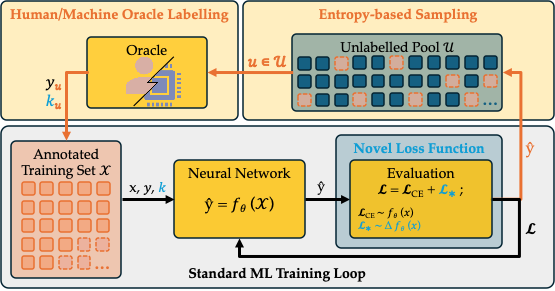
\includegraphics[width=0.8\textwidth]{figures/diagram.png}
  \caption{Overview of the proposed counterfactually-augmented active learning framework. 
  The model leverages both factual and counterfactual samples, selected via importance sampling, and trained using a hybrid loss function.}
  \label{fig:method_overview}
\end{figure*}


\label{sec:gradient_learning}

\subsection{Interactive Annotation Interface}
\label{subsec:annotation_interface}

The annotation scheme described in this chapter requires a mechanism by which a human expert can (a) inspect how the model is behaving and (b) supply counterfactual direction annotations in a form the training pipeline can consume. Figure~\ref{fig:method-pipeline} contrasts the traditional supervised learning pipeline with our proposed interactive extension: rather than treating annotation as a one-time offline step, the annotator can pause training at any point, examine the current decision surface, add or refine direction vectors for any observations, and then resume training. This cycle can be repeated indefinitely, and the model need never see new labelled examples.

\begin{figure}[t]
    \centering
    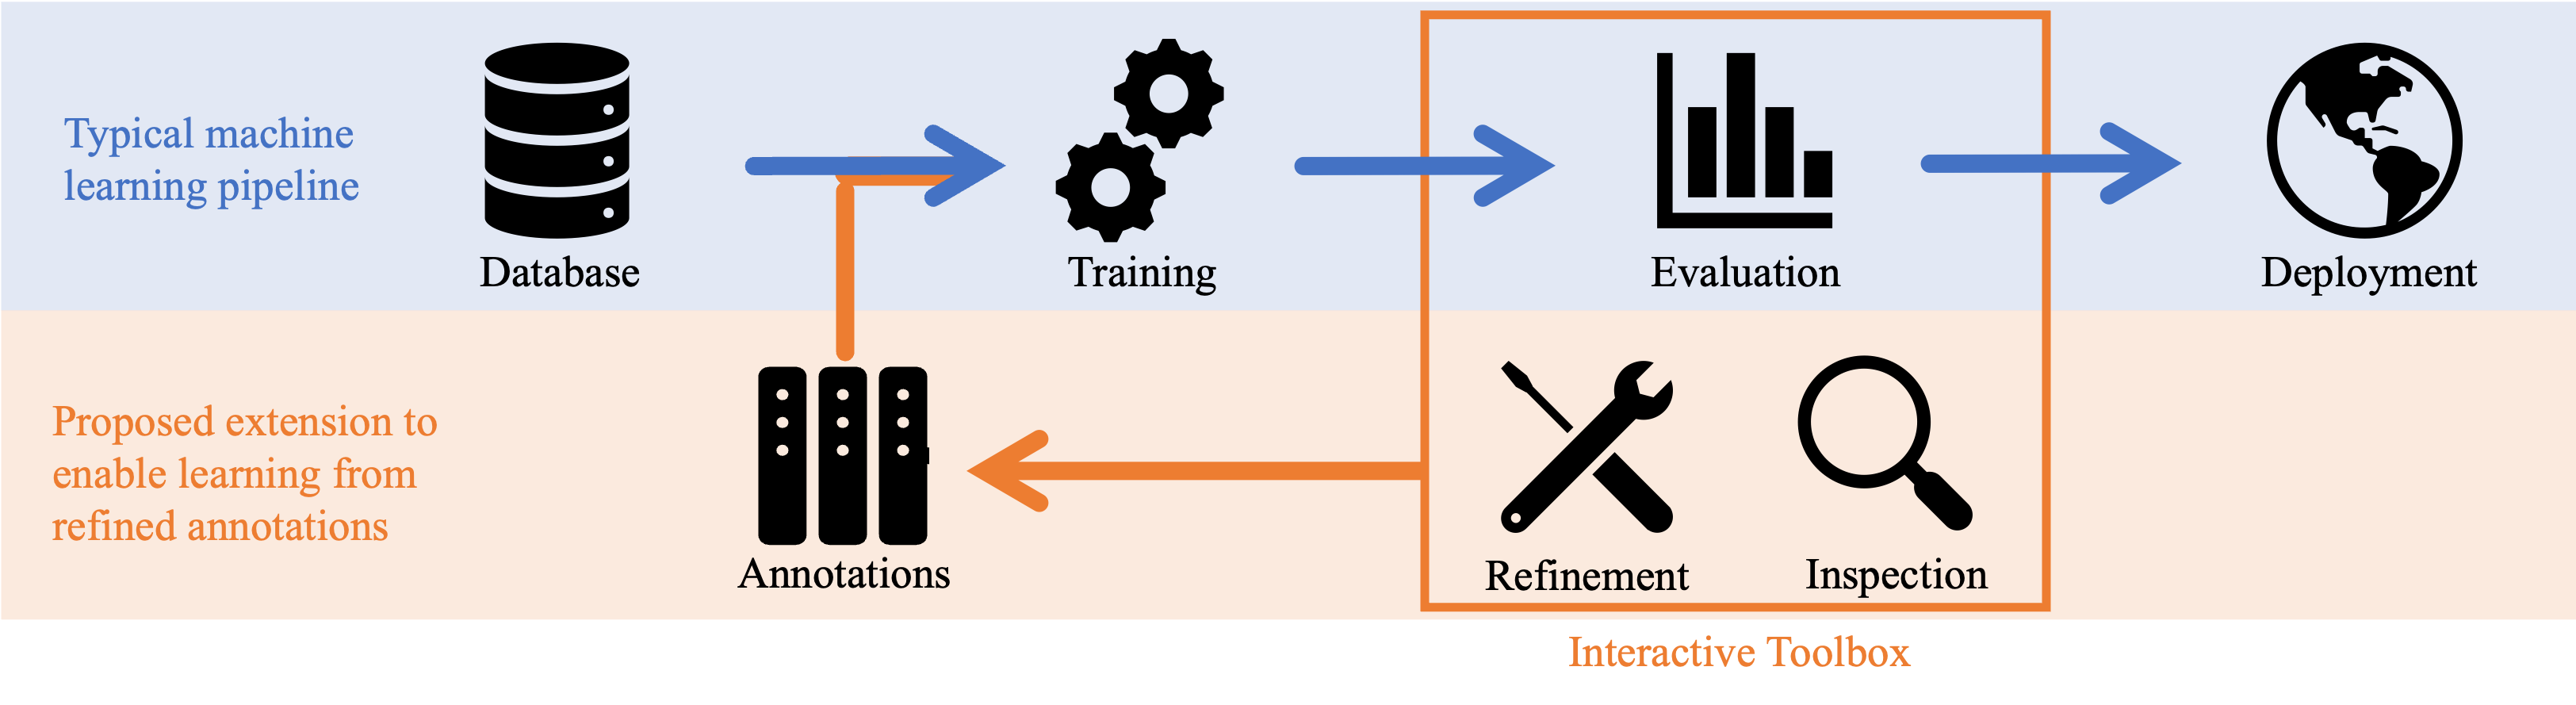
\includegraphics[width=\linewidth]{figures/gui_pipeline_IJCAI}
    \caption{The traditional supervised learning pipeline (top) contrasted with our proposed interactive human-in-the-loop method (bottom). The annotator can pause training, inspect the evolving decision surface, and supply counterfactual direction annotations before resuming.}
    \label{fig:method-pipeline}
\end{figure}

The graphical user interface through which these annotations are collected is shown in Figure~\ref{fig:method-gui}. The \emph{inspection console} (centre) presents a live visualisation of the dataset overlaid with the model's predicted probability surface and decision boundary, updated during training so the annotator can observe where the model is currently incorrect. The \emph{evaluation console} (top) tracks test accuracy over time and supports side-by-side comparison of multiple saved experiments, allowing the effect of different annotation strategies to be assessed directly. The \emph{annotation toolbox} (lower left) enables the expert to select any training point and draw one or more arrows indicating the counterfactual direction $\mathbf{d}_i$; existing annotations are shown in black and the one currently being drawn in green.

\begin{figure}[t]
    \centering
    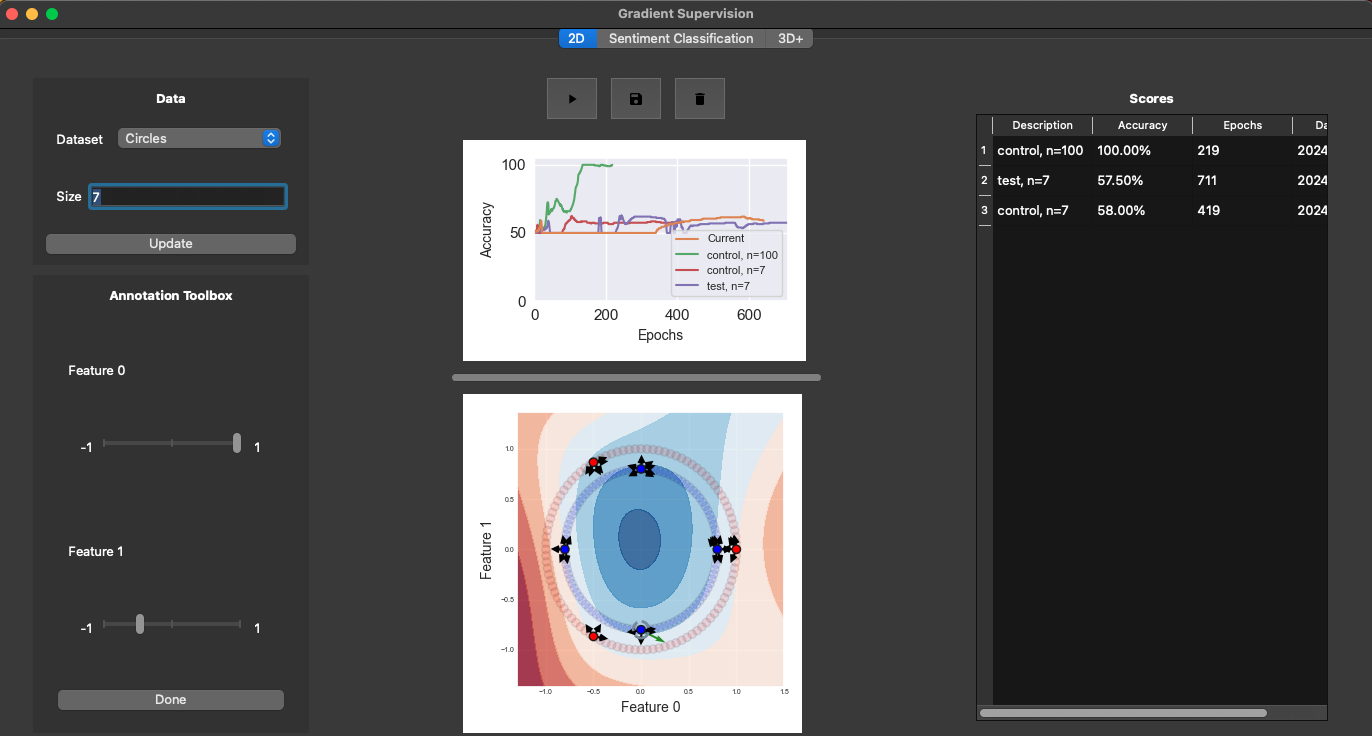
\includegraphics[width=\linewidth]{figures/gui_wide}
    \caption{The Graphical User Interface (GUI) for interactive counterfactual annotation~\cite{erskine2024ijcai}. The annotation toolbox (lower left) lets the expert draw direction vectors $\mathbf{d}_i$ for selected data points. The inspection console (centre) shows the live decision surface relative to training (solid) and test (transparent) examples. The evaluation console (top) tracks and compares test accuracy across experiments. The example shows a nine-observation run: the control (no annotations) and an annotated version whose directions are visible in the inspection console.}
    \label{fig:method-gui}
\end{figure}

This annotation scheme is intentionally domain-agnostic: any form of human feedback that can be encoded as a direction in feature space can replace the arrow-drawing interaction, and the accompanying loss function can be swapped accordingly. The interface source code and a user manual are available at \url{https://github.com/jmerskine1/interactive_gradients}. The formal representation of these annotations and the loss functions that consume them are defined in the subsections that follow.

\subsection{Directional Expert Annotation}
In traditional supervised machine learning, we assume a dataset of $N$ random independent identically distributed (i.i.d.) observations {$\mathbf{x_i}, y_i$} $\sim P(\mathbf{x},y)$, where $\mathbf{x_i}\in\mathcal{R}^d$ and $y_i$ is the target class label \cite{hastie2009elements}. In the CGA framework, we consider triplets {$\mathbf{x_i}, y_i, \mathbf{d_i}$}, where $\mathbf{d_i} \in \mathcal{R}^d$ defines a unit vector from $\mathbf{x_i}$ pointing towards a proximal counterfactual $\hat{\mathbf{x}}_i$: 
\begin{equation}
    \mathbf{d_i}=\frac{\hat{\mathbf{x}}_i - \mathbf{x_i}}{||\hat{\mathbf{x}}_i - \mathbf{x_i}||}. \label{eq:dir_unit}
\end{equation}

We propose that moving from $\mathbf{x_i}$ towards $\hat{\mathbf{x}}_i$ should result in a decrease in the model's prediction probability for the true class $y$. Let $f_y(\mathbf{x})$ be the model's logit score for class $y$. We define the \textbf{Directional Derivative} $d$ as the projection of the gradient onto the counterfactual direction:
\begin{equation}
    d = \nabla_x f_{y}(x) \cdot \mathbf{d}_{i}
\end{equation}
This derivative quantifies how much the class confidence changes as we perturb the input along the expert-provided direction.


\begin{figure}
    \centering
    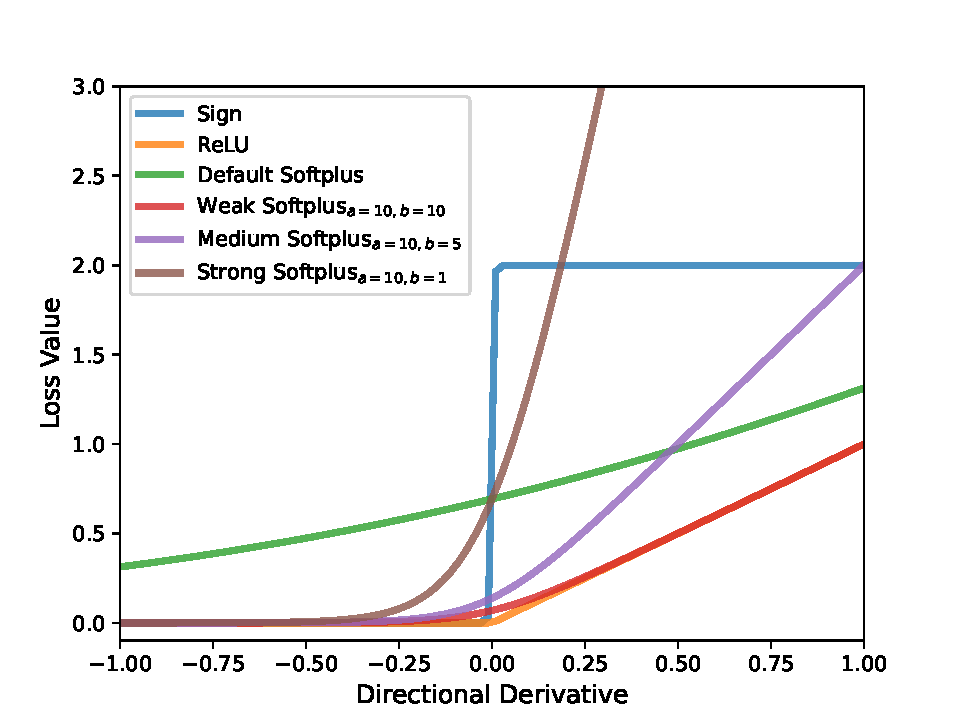
\includegraphics[width=\linewidth]{figures/loss_functions_comparison.pdf}
    % \caption{}
    \caption{Comparison of the three directional loss variants $\mathcal{L}_{\text{Sign}}$, $\mathcal{L}_{\text{ReLU}}$, and $\mathcal{L}_{\text{Softplus}}$ as functions of the directional derivative $d$. The Sign loss provides a steep, bounded penalty based only on the gradient sign, the ReLU loss applies a linear penalty for positive (misaligned) gradients, and the Softplus loss offers a smooth, tunable alternative that can still impose a non-zero penalty even when $d$ is negative, depending on its magnitude.}
    \label{fig:losses}
\end{figure}

\subsection{Optimized Loss Function Variants}
We evaluate three loss variants $\mathcal{L}_{d}$ designed to minimize $d$, aligning the model's confidence drop with the counterfactual path. The intuition is that $d$ should be negative at the counterfactual direction, with each variant modifying the profile of this negative loss in terms of magnitude and steepness.

\paragraph{Sign (Tanh) Directional Loss}
The purest form of our proposed loss function penalises only the sign of the model gradient; disregarding negative model gradients and generating a fixed loss penalty for positive model gradients, regardless of the magnitude of the gradient. This loss was first introduced alongside the interactive interface in~\cite{erskine2024ijcai} and serves as the starting point for the richer variants below.
The Sign variant is formulated as:
\begin{equation}
    \mathcal{L}_{\text{Sign}} = \tanh(200*d) + 1
\end{equation}
where the high multiplier creates a very steep tanh function, squashing the derivative into the range $\mathcal{L}_{\text{Sign}} \in [0,2]$. We hypothesise that focusing purely on the sign of the alignment ensures a bounded, stable regularising signal across different manifolds.


\paragraph{ReLU Directional Loss}
\begin{equation}
    \mathcal{L}_{\text{ReLU}} = \max(0, d)
\end{equation}
This applies a linear penalty only if the model's confidence is incorrectly \emph{increasing} toward the counterfactual boundary. It is a "hinge-like" objective that stops regularizing once the gradient sign is correct. By attributing higher penalties to steeper positive gradients, this function is more communicative, but may prove to be over-restrictive, particularly for noisy datasets.

\paragraph{Softplus Directional Loss}
Softplus is a smooth version of ReLU that provides a continuous alignment signal. Unlike ReLU, it can provide a non-zero penalty even when $d$ is negative dependent on the magnitude of the derivative. While this may encourage the model to maintain a "steep" confidence drop-off even when it is already locally "correct", it is unclear how informative this signal will be, particularly in sparse regimes. We therefore utilise a modified Softplus function defined as:
\begin{equation}
    \mathcal{L}_{\text{Softplus}} = \log(1 + e^{ad})/b
\end{equation}
where $a$ controls the steepness of the penalty and $b$ normalises its magnitude. In our experiments we evaluate three configurations: \emph{Softplus-Weak} ($a=1, b=2$), \emph{Softplus-Medium} ($a=5, b=5$), and \emph{Softplus-Strong} ($a=20, b=10$), providing a sweep from a gentle, near-linear penalty to a steep signal approaching the Sign variant. Figure~\ref{fig:losses} compares the behaviour of each loss function variant across this range.


\subsection{Total Training Objective} 

The total training loss is a weighted mixture of classification and alignment objectives:

\begin{equation}\label{eq:total_loss}
\mathcal{L}_{\text{Total}} = (1-\alpha)\mathcal{L}_{\text{CE}} + \alpha \left( \frac{1}{N_d} \sum^{N_d}_{i=1} \mathcal{L}_{d,i} \right)
\end{equation}

where $N_d$ is the number of examples in the training set for which we have labelled directions, and $\alpha \in [0,1]$ controls the trade-off between standard classification and geometric supervision. When $\alpha = 0$ the objective reduces to standard cross-entropy, providing a natural baseline. Note that the directional loss is only applied to annotated examples; unannotated examples contribute only the cross-entropy term, so the framework degrades gracefully when counterfactual coverage is sparse.

\subsection{Informative and Diverse Sample Selection}
To maximize the utility of human-in-the-loop annotations under data scarcity, we employ a hybrid importance sampling strategy that balances \textit{informativeness} (via entropy) and \textit{diversity} (via geometric distance). This approach addresses a known failure mode of pure uncertainty sampling: the redundancy problem, where a model selects high-entropy samples that are spatially clustered, leading to overlapping and inefficient gradient updates~\cite{shen2018deepactivelearningnamed}.

Our selection mechanism follows a two-stage process. First, we identify a candidate pool of the most informative samples based on Shannon entropy, $H(p) = -\sum p_i \log p_i$. To ensure this subset provides broad coverage of the feature manifold, we apply a greedy selection process inspired by the K-Center-Greedy approach~\cite{sener2018activelearning}. For each candidate $x$ in the high-entropy pool, we compute a selection score:
\begin{equation}
    \text{score}(x) = H(x) + \alpha \cdot \min_{s \in \mathcal{S}} \| \phi(x) - \phi(s) \|_2
\end{equation}
where $\mathcal{S}$ is the set of already selected samples, $\phi(\cdot)$ denotes the embedding function, and $\alpha$ is a diversity weight. 

This weighted hybrid formulation, as explored in batch active learning~\cite{citovsky2021batchactivelearningscale}, ensures that each selected sample is both locally uncertain and globally distant from existing annotations. By employing this strategy, we ensure that the counterfactual direction annotations enrich the model across a diverse range of the data distribution, which is critical for effective supervision when annotation budgets are strictly limited.


\section{Experimental Setup}
\label{sec:experimental_setup}
Our method is applicable to any dataset for which counterfactual directions can be defined, either by direct generation or human annotation. We validate across two complementary domains. First, we evaluate on four synthetic 2D classification tasks for which ground-truth counterfactuals can be generated automatically, allowing precise control over dataset size and counterfactual coverage. Second, we evaluate on two natural language classification tasks: (1) binary sentiment classification on IMDB movie reviews, using \emph{human-generated} counterfactuals collected by \citet{Kaushik2020Learning}, and (2) four-class topic classification on the AGNEWS news article dataset~\cite{NIPS2015_250cf8b5}, using machine-generated counterfactuals. Together these settings probe the framework across low-dimensional geometric and high-dimensional lexical feature spaces.


\subsection{Datasets}
The objective of our experiments is to measure how incorporating counterfactuals using Eq.~\ref{eq:total_loss} may improve data efficiency. To this end we utilise small subsets of the available training data to simulate data scarcity, a common challenge in real-world applications, and report results for training sets of various sizes. In all experiments we compare our method against the gradient supervision model proposed by \citet{teney2020learning} (replacing $\mathcal{L}_d$ in Eq~\ref{eq:total_loss}) and a baseline model trained on cross-entropy (Eq.~\ref{eq:total_loss}, $\alpha=0$).


\begin{table}[h]
\centering
\caption{Dataset Split Sizes.}
\label{tab:all_datasets}
\begin{tabular}{lrrr}
\toprule
\textbf{Dataset} & \textbf{Train} & \textbf{Validation} & \textbf{Test} \\ 
\midrule
\textit{Synthetic 2D} & & & \\
Circles   & 6     & 1,000 & --    \\
XOR       & 6     & 1,000 & --    \\
Two Moons & 6     & 1,000 & --    \\
9-Blobs   & 60    & 1,000 & --    \\ 
\midrule
\textit{NLP Classification} & & & \\
IMDB      & 1,707 & 245   & 488   \\
AGNEWS    & 500   & 3,550 & 3,550 \\ 
\bottomrule
\end{tabular}
\end{table}

\subsubsection{2D Topologies}
We evaluate our method across four synthetic 2-dimensional topologies generated using the \texttt{scikit-learn} library~\citep{scikit-learn}. These consist of three binary classification tasks—XOR, Concentric Circles, and Two Moons—and a more complex multi-class objective featuring nine classes of distinct Gaussian clusters. This selection allows us to assess the framework's performance on both interleaved non-linear boundaries and high-entropy multi-class partitions. Counterfactuals are generated using a brute force grid search, implemented with the FAT Forensics toolkit \cite{sokol2020fat-forensics}. We first tune the model hyperparameters and dataset size on the cross-entropy baseline, finding the minimal amount of data to fully learn the problem and then marginally reducing the dataset further to introduce epistemic uncertainty. We train with relatively small subsets of data and omit a test set in lieu of a suitably large validation set. Training and validation set sizes are given in Table~\ref{tab:all_datasets}. To compare data efficiency between counterfactuals and simply learning from additional labels, we also introduce an \textbf{upper bound baseline which is trained on twice as many examples}.




\paragraph{Model Architecture} For these 2D datasets, we utilize an overparameterized Multi-Layer Perceptron (MLP) consisting of a single hidden layer with 512 units and \texttt{ReLU} activation. While this width is high relative to the input dimensionality, we observe that overparameterization consistently boosts validation accuracy on the control model trained with cross-entropy and provides a high-dimensional feature space conducive to geometric alignment. The model is optimized using the \textbf{AdaBelief} optimizer~\citep{zhuang2020adabeliefoptimizeradaptingstepsizes} with $\beta_1{=}0.9$, $\beta_2{=}0.999$, and $\epsilon{=}1^{-16}$, with the learning rate $l = 0.001$.

\subsubsection{Natural Language}
We utilise two openly available text datasets which provide counterfactual examples alongside training data for binary sentiment classification on movie reviews (IMDB) and topic classification for news articles (AGNEWS). Table~\ref{tab:all_datasets} gives the sizes of available data for training, validation and testing for each dataset. For IMDB, we utilised the human-generated counterfactually-augmented dataset curated by \citet{Kaushik2020Learning}, maintaining separation of the test set into the original and augmented reviews as in the original work\cite{Kaushik2020Learning}. For AGNEWS, we utilised machine-generated counterfactuals generated by \citet{wang2025truthtwistoptimalmodel}. In their study, \citet{wang2025truthtwistoptimalmodel} evaluate several generative models with both machine and human evaluators. To investigate potential variance from counterfactual quality, we evaluate two sets of counterfactually-augmented data:
\begin{enumerate}
    \item Counterfactuals generated by (1) Llama3-70B using the FIZLE generation methodology\cite{FIZLE} for which label flip score (LFS) is well aligned between human and machine evaluators; $63.6\%$ and $64.4\%$ respectively.
    \item Counterfactuals generated by Llama3-8B using the more polarising FLARE methodology \cite{FLARE} which achieves only $42.2\%$ LFS against a machine judge and a much higher $86.7\%$ for humans.
\end{enumerate}


\paragraph{Data Preprocessing}
All text datasets were stripped of HTML, bracketed content, URLs, email addresses, and numbers, followed by tokenization into lowercase words, stopword removal, and rule-based stemming to normalize lexical forms. 

\paragraph{Feature Representation}
A \texttt{CountVectorizer} was fitted to the training corpus, limited to the 20,000 most frequent tokens. This vocabulary was then reused for both development and test sets. Each document was transformed into a fixed-length sequence of token indices mapped to the vocabulary, truncated or padded to a length of 32. This truncation is intentionally aggressive: as the model uses average pooling over token embeddings, the pooled representation is largely stable beyond a moderate context window, and shorter sequences reduce memory and compute cost in the low-data regime of interest.

\paragraph{Model Architecture}
For text classification, we employed a \textbf{Bag-of-Words (BoW)} neural network implemented in \texttt{JAX/Flax}. Two model variants were used depending on the task: a binary classifier (\texttt{BagOfWordsClassifierSimple}) and a multi-class classifier (\texttt{BagOfWordsClassifierMultiClass}). Both models share the same general structure:
\begin{enumerate}
\item \textbf{Embedding layer:} A trainable embedding matrix maps token indices to dense vectors of dimension 50.
\item \textbf{Average pooling:} Embeddings for all tokens in a document are averaged, ignoring padding tokens.
\item \textbf{Dropout:} A dropout layer (rate = 0.5) is applied to mitigate overfitting.
\item \textbf{Linear projection:} A single dense layer maps the pooled representation to either one logit (binary classification) or $N$ logits (multi-class classification).
\end{enumerate}
The model outputs both the predicted logits and the intermediate text representation, which are used for downstream tasks such as similarity computation and importance sampling.


% 
\subsubsection{Image Classification}
Describe data prep and model architecture


In our framework, we employ multiple approaches to generate counterfactual paths, moving beyond simple shortest-distance methods to incorporate more sophisticated path-finding strategies that ensure both feasibility and actionability. \todo[inline]{provide figure showing comparison}

\paragraph{Feasible Path Generation}
Drawing from the work of Sokol et al. on navigating explanatory multiverse through counterfactual path geometry~\cite{sokol2023navigating}, we implement feasible path generation. This approach aims to address two critical limitations of traditional counterfactual methods: ensuring the counterfactual instance lies within high-density regions of the data distribution, and guaranteeing the existence of a plausible transformation path from the original instance.

The feasible path generation process utilizes density-weighted graph construction, where edge weights incorporate both distance metrics and local data density information. This approach ensures that generated paths traverse high-density regions of the feature space, making the resulting counterfactuals more representative of the underlying data distribution~\cite{poyiadzi2020face}. In this work we aim to evaluate how useful these counterfactuals are compared to counterfactuals generated by the shortest path baselines.

\paragraph{Shortest Path Baselines}

To evaluate the effectiveness of feasible path strategies, we implement two baseline approaches based on shortest-distance metrics: raw Euclidean distance and PCA-transformed distance. These baselines provide comparison points for understanding when sophisticated path-finding offers advantages over simpler geometric approaches.


\paragraph{Feature Representation}
Images are provided as flattened grayscale inputs derived from the original ($28 \times 28$) MNIST digits, with pixel intensities normalised to the range ($[0, 1]$).

\paragraph{Model Architecture}
For image classification, we employed a \textbf{Convolutional Neural Network (CNN)} implemented in \texttt{JAX/Flax}. The model, denoted \texttt{MNISTConvClassifierGemini}, extracts spatial features from grayscale images and maps them to class predictions. Its architecture consists of the following components:
\begin{enumerate}
\item \textbf{Convolutional feature extractor:} Two convolutional layers with 32 and 64 filters (kernel size $3 \times 3$) are each followed by ReLU activation and max-pooling ($2 \times 2$).
\item \textbf{Feature embedding:} The flattened feature maps are projected into a 512-dimensional dense representation.
\item \textbf{Dropout regularization:} A dropout layer (rate = 0.4) is applied to the embedding during training to mitigate overfitting.
\item \textbf{Classification head:} A final dense layer maps the embedding to ten output logits corresponding to the MNIST digit classes.
\end{enumerate}
Convolutional layers use LeCun-normal initialization, while dense layers use Glorot-normal initialization. The model outputs both class logits and the intermediate feature embeddings for use in downstream analyses. All hyperparameters are optimised on the validation set for experiments with cross-entropy.

\subsection{Ablation Study and Importance Sampling}
For our 2D experiments, we provide a counterfactual on a per-example basis. We then test all loss function variants across all problems, varying $\alpha$ to modify the influence of our loss function. After optimising on the 2D datasets, we fix $\alpha$ and select the most effective variant of our proposed loss function to perform experiments within the NLP setting. To understand the relationship between counterfactual annotations and information gain we randomly ablate generated counterfactuals to some ratio $r \in [0,1]$ of total training examples \textbf{in the NLP setting only}. Our interest in low-data regimes motivates further investigation whereby we perform importance sampling; we repeat each NLP experiment starting from 10\% of available data, iteratively selecting 5\% unlabelled observations and adding these to the training data every 2 training epochs before re-initialising the model and re-training. We run for the same amount of epochs as the 'AL Off' scenario as we are mainly interested in data efficiency in earlier epochs. Data selection is performed by balancing label uncertainty and sample diversity. A full description of our sampling strategy is provided in Appendix~\ref{appendix:al}.

% %%%%%%%%%%%%%%%%%%%%%%%%%%%%%%%%%%%%%%%%%%%%%%%%%%%%%%%%%%%%%%%%%%%%%%%%%%%%%%%%%%%
% % Results
% %%%%%%%%%%%%%%%%%%%%%%%%%%%%%%%%%%%%%%%%%%%%%%%%%%%%%%%%%%%%%%%%%%%%%%%%%%%%%%%%%%%
\section{Results}
\label{sec:results}

\begin{table*}[ht]
\centering
\caption{Validation Accuracy (\%) and Epochs for 2D Classification Tasks trained with and without counterfactuals, using different loss function variants while varying the relative strength of the supervisory signal ($\alpha \in [0,1] $). Bold values show the best accuracy for that specific loss function variant, while \globalbest{Underlined Bold} shows the best accuracy across the entire experiment. \fastest{Epochs in bold} indicate that the run is the \textbf{most efficient} in its group, but \underline{only} if it is also the \textbf{most accurate}. An upper bound is trained on twice as much data, to allow comparison of data efficiency between learning from counterfactuals or simply adding more labelled examples.}  
\label{tab:results_alpha_variants}

\resizebox{\textwidth}{!}{%
\begin{tabular}{ll cc cc cc cc}
\toprule
& & \multicolumn{2}{c}{\textbf{Circles}} & \multicolumn{2}{c}{\textbf{XOR}} & \multicolumn{2}{c}{\textbf{Two Moons}} & \multicolumn{2}{c}{\textbf{9-Blobs}} \\
\cmidrule(lr){3-4} \cmidrule(lr){5-6} \cmidrule(lr){7-8} \cmidrule(lr){9-10}
\textbf{Variant} & $\alpha$ & \% Acc & Ep & \% Acc & Ep & \% Acc & Ep & \% Acc & Ep \\
\midrule
Baseline ($\mathcal{L}_{\text{CE}}$) & 0.0 & 87.8 (±0.054) & 35 & 99.1 (±0.001) & 86 & 77.3 (±0.003) & 18 & 84.8 (±0.002) & 194 \\
\rowcolor{gray!15} Upper Bound  ($\mathcal{L}_{\text{CE}}$)  & 0.0 & 100.0\% (±0.029) & 37 & 100.0\% (±0.002) & 35 & 86.6\% (±0.001) & 58 & 85.8\% (±0.004) & 162 \\
\midrule
\multirow{3}{*}{Gradient Supervision} 
    & 0.3 & \textbf{74.7 (±0.027)} & \fastest{74} & 99.7 (±0.001) & 78 & \textbf{85.7 (±0.031)} & 95 & \textbf{85.8 (±0.004)} & 162 \\
    & 0.5 & 74.2 (±0.020) & 76 & 99.7 (±0.001) & 65 & 81.3 (±0.008) & 46 & 85.4 (±0.003) & 123 \\
    & 0.7 & 74.4 (±0.019) & 85 & \textbf{\globalbest{99.8 (±0.001)}} & 88 & 80.4 (±0.035) & 37 & 85.1 (±0.001) & 187 \\
\midrule
\multirow{3}{*}{Sign} 
    & 0.3 & \textbf{80.9 (±0.078)} & \fastest{36} & 95.9 (±0.028) & 99 & 77.0 (±0.014) & 17 & 86.4 (±0.016) & 197 \\
    & 0.5 & 80.4 (±0.068) & 47 & \textbf{97.2 (±0.036)} & \fastest{99} & 77.0 (±0.016) & 8 & \textbf{87.1 (±0.016)} & 196 \\
    & 0.7 & 80.6 (±0.065) & 47 & 95.7 (±0.054) & 99 & \textbf{77.5 (±0.011)} & 13 & 86.3 (±0.024) & 191 \\
\midrule
\multirow{3}{*}{ReLU} 
    & 0.3 & \textbf{\globalbest{90.2 (±0.062)}} & 44 & \textbf{99.5 (±0.002)} & \fastest{72} & 78.8 (±0.006) & 13 & 87.0 (±0.006) & 196 \\
    & 0.5 & 88.5 (±0.046) & 40 & \textbf{99.5 (±0.002)} & 78 & 79.0 (±0.010) & 8 & 87.6 (±0.002) & 195 \\
    & 0.7 & 85.4 (±0.062) & 39 & 99.5 (±0.004) & 95 & \textbf{79.8 (±0.013)} & \fastest{5} & \textbf{88.6 (±0.007)} & \fastest{190} \\
\midrule
\multirow{3}{*}{Softplus-Weak} 
    & 0.3 & 87.2 (±0.041) & 43 & 99.5 (±0.001) & 66 & 80.2 (±0.005) & 21 & 87.5 (±0.005) & 199 \\
    & 0.5 & 86.7 (±0.035) & 50 & 99.5 (±0.001) & 70 & 81.2 (±0.005) & 12 & 88.7 (±0.006) & 190 \\
    & 0.7 & \textbf{88.2 (±0.075)} & 99 & \textbf{99.6 (±0.001)} & 88 & \textbf{82.8 (±0.018)} & \fastest{4} & \textbf{89.2 (±0.004)} & \fastest{159} \\
\midrule
\multirow{3}{*}{Softplus-Medium} 
    & 0.3 & 87.0 (±0.035) & 49 & 99.5 (±0.001) & 69 & 81.1 (±0.004) & 13 & 88.4 (±0.006) & 194 \\
    & 0.5 & \textbf{88.6 (±0.081)} & 99 & \textbf{99.6 (±0.001)} & 92 & 82.3 (±0.018) & 4 & 89.0 (±0.006) & 173 \\
    & 0.7 & 88.4 (±0.028) & 99 & \textbf{99.6 (±0.001)} & 91 & \textbf{84.6 (±0.030)} & \fastest{2} & \textbf{89.1 (±0.008)} & \fastest{130} \\
\midrule
\multirow{3}{*}{Softplus-Strong} 
    & 0.3 & \textbf{\globalbest{90.2 (±0.044)}} & 168 & 99.6 (±0.002) & 89 & 84.6 (±0.024) & 3 & 88.9 (±0.005) & 139 \\
    & 0.5 & 82.5 (±0.041) & 27 & \textbf{99.7 (±0.003)} & 96 & \textbf{\globalbest{86.3 (±0.026)}} & \fastest{3} & \textbf{\globalbest{89.3 (±0.004)}} & 192 \\
    & 0.7 & 82.1 (±0.080) & 26 & 99.5 (±0.004) & 99 & 85.5 (±0.011) & 5 & \textbf{\globalbest{89.3 (±0.004)}} & 183 \\
\bottomrule
\end{tabular}
}
\end{table*}



\subsection{2D Experiments}
Table~\ref{tab:results_alpha_variants} shows results for these experiments. Across all four topologies, incorporating counterfactual supervision (either through gradient supervision or a CGA variant) yields faster convergence, higher accuracy, or both, relative to the cross-entropy baseline. This is consistent with the hypothesis that directional annotations provide a richer learning signal than labels alone. Notably, for \textbf{Two Moons} and \textbf{9-Blobs}, several CGA variants exceed the upper bound accuracy despite using only half as many training examples. In the case of \textbf{Two Moons}, \emph{Softplus-Strong} matches the upper bound accuracy whilst requiring fewer than $10\%$ of the epochs. For \textbf{9-Blobs}, all proposed CGA variants surpass the upper bound, suggesting that directional supervision can compensate for reduced data more effectively than simply providing additional labels. The best-performing variant is inconsistent across topologies, indicating a sensitivity to dataset geometry that is explored further in the Discussion.

%
% NLP
%

\subsection{NLP Classification Tasks}

%start of paste
\subsubsection{IMDB}
Table~\ref{tab:results_imdb_al_off} and Table~\ref{tab:results_imdb_al_on} show results for sentiment classification on the IMDB dataset for the case of full data availability and the active learning setting respectively. At $N=20$ (and extending to $N=50$ under the active learning paradigm), all variant collapse to a baseline accuracy of 52.9\% at Epoch 0. This indicates that for this specific architecture and task, 20 to 50 samples are simply insufficient to overcome initial random initializations, regardless of the loss function variant applied.

As the dataset scales to $N=100$ and $N=500$, the Gradient Supervision (GS) variant with $r=1.0$ and the standard Cross-Entropy (C.E.) baseline consistently outpace the Softplus-Strong alternative. In the standard AL Off setting, GS ($r=1.0$) edges out C.E.\ to achieve the global best accuracy at both $N=100$ (63.1\%) and $N=500$ (75.8\%). Softplus-Strong, conversely, lags behind the baseline by nearly 8\% at $N=500$.

We observe a strict sensitivity to the mixing parameter $r$ within the GS framework. While $r=1.0$ yields peak performance, reducing the ratio to $r=0.5$ triggers catastrophic forgetting or learning failure; at $N=500$ (AL Off), accuracy drops from 75.8\% down to a near-baseline 53.9\%. 

In the active learning setting, neither method is able to surpass the baseline model trained with cross-entropy. However, for $N=100$, both counterfactual methods approximate the baseline accuracy whilst requiring approximately $50\%$ fewer training epochs, with the CGA loss converging slightly faster than gradient supervision.

%
% IMBD
%
\begin{table*}[ht]
\centering
\caption{Test Accuracy (\%) and Epochs on IMDB (AL Off). For loss functions which utilise counterfactuals we fix the parameter, $\alpha = 0.5$. Bold values show the best accuracy for that specific loss function variant, while \globalbest{Underlined Bold} shows the best accuracy across the entire experiment. \fastest{Epochs in bold} indicate that the run is the \textbf{most efficient} in its group, but \underline{only} if it is also the \textbf{most accurate}.}
\label{tab:results_imdb_al_off}

\resizebox{\textwidth}{!}{%
\begin{tabular}{ll cc cc cc cc}
\toprule
& & \multicolumn{8}{c}{\textbf{Dataset Size}} \\
\cmidrule(lr){3-10}
& & \multicolumn{2}{c}{\textbf{20}} & \multicolumn{2}{c}{\textbf{50}} & \multicolumn{2}{c}{\textbf{100}} & \multicolumn{2}{c}{\textbf{500}} \\
\cmidrule(lr){3-4} \cmidrule(lr){5-6} \cmidrule(lr){7-8} \cmidrule(lr){9-10}
\textbf{Variant} & \textbf{r} & \% Acc & Ep & \% Acc & Ep & \% Acc & Ep & \% Acc & Ep \\
\midrule
C.E. & - & 52.9 (±0.033) & 0 & 50.4 (±0.002) & 55 & 62.9 (±0.005) & 51 & 75.4 (±0.003) & 14 \\
\midrule
\multirow{2}{*}{GS} 
    & 1.0 & 52.9 (±0.033) & 0 & 50.4 (±0.002) & 56 & \textbf{\globalbest{63.1 (±0.004)}} & 45 & \textbf{\globalbest{75.8 (±0.004)}} & 14 \\
    & 0.5 & 52.9 (±0.033) & 0 & \textbf{\globalbest{54.3 (±0.016)}} & \fastest{18} & 54.3 (±0.024) & 5 & 53.9 (±0.027) & 0 \\
\midrule
\multirow{2}{*}{Softplus-Strong} 
    & 1.0 & 52.9 (±0.033) & 0 & \textbf{49.8 (±0.006)} & \fastest{1} & \textbf{57.6 (±0.008)} & 53 & \textbf{67.6 (±0.009)} & \fastest{22} \\
    & 0.5 & 52.9 (±0.033) & 0 & \textbf{49.8 (±0.005)} & \fastest{1} & 56.8 (±0.006) & 52 & 66.8 (±0.012) & 33 \\
\bottomrule
\end{tabular}
}
\end{table*}


\begin{table*}[ht]
\centering
\caption{Test Accuracy (\%) and Epochs on IMDB (AL On). For loss functions which utilise counterfactuals we fix the parameter, $\alpha = 0.5$. Bold values show the best accuracy for that specific loss function variant, while \globalbest{Underlined Bold} shows the best accuracy across the entire experiment. \fastest{Epochs in bold} indicate that the run is the \textbf{most efficient} in its group, but \underline{only} if it is also the \textbf{most accurate}.}
\label{tab:results_imdb_al_on}

\resizebox{\textwidth}{!}{%
\begin{tabular}{ll cc cc cc cc}
\toprule
& & \multicolumn{8}{c}{\textbf{Dataset Size}} \\
\cmidrule(lr){3-10}
& & \multicolumn{2}{c}{\textbf{20}} & \multicolumn{2}{c}{\textbf{50}} & \multicolumn{2}{c}{\textbf{100}} & \multicolumn{2}{c}{\textbf{500}} \\
\cmidrule(lr){3-4} \cmidrule(lr){5-6} \cmidrule(lr){7-8} \cmidrule(lr){9-10}
\textbf{Variant} & \textbf{r} & \% Acc & Ep & \% Acc & Ep & \% Acc & Ep & \% Acc & Ep \\
\midrule
C.E. & - & 52.9 (±0.033) & 0 & 52.9 (±0.033) & 0 & \textbf{\globalbest{58.8 (±0.004)}} & 94 & \textbf{\globalbest{72.3 (±0.002)}} & 81 \\
\midrule
\multirow{2}{*}{GS} 
    & 1.0 & 52.9 (±0.033) & 0 & 52.9 (±0.033) & 0 & \textbf{58.6 (±0.006)} & 67 & \textbf{71.5 (±0.003)} & 83 \\
    & 0.5 & 52.9 (±0.033) & 0 & 52.9 (±0.033) & 0 & 53.7 (±0.023) & 63 & 53.5 (±0.018) & 9 \\
\midrule
\multirow{2}{*}{Softplus-Strong} 
    & 1.0 & 52.9 (±0.033) & 0 & 52.9 (±0.033) & 0 & \textbf{57.8 (±0.007)} & \fastest{61} & \textbf{67.4 (±0.005)} & 94 \\
    & 0.5 & 52.9 (±0.033) & 0 & 52.9 (±0.033) & 0 & 57.0 (±0.006) & 98 & 66.6 (±0.003) & 73 \\
\bottomrule
\end{tabular}
}
\end{table*}

%
% AGNEWS
%
\subsubsection{AGNEWS}

Table~\ref{tab:results_fizle_flare_al_off_stacked} and Table~\ref{tab:results_fizle_flare_al_on_stacked} present the validation accuracies for the AGNEWS text classification dataset, evaluated across the FIZLE and FLARE experimental subsets for both standard (AL Off) and active learning (AL On) sampling strategies.

Consistent with our previous NLP observations, an extreme low-data bottleneck exists at $N=20$, where all models fail to exceed the 24.2\% baseline (random chance across the four AGNEWS classes). However, a significant divergence occurs at the $N=50$ threshold under standard uniform sampling (AL Off). Here, the Softplus-Strong ($a=0.5$) variant demonstrates exceptional sample efficiency, leaping to a global best of 44.9\% (FIZLE) and 48.7\% (FLARE) with $r=0.5$, while the Cross-Entropy (C.E.) baseline stagnates around 30.2\%. As the dataset scales to $N=100$ and $N=500$, the Softplus-Strong variant with $r=1.0$ produces the best results, although the discrepancy is smaller. Importantly, we note only a marginal reduction in performance when utilising half as many counterfactuals for our loss variant (at $N=50$ we actually improve by reducing counterfactual annotations). The gradient supervision method is markedly more sensitive to ablation.

Across almost all viable training scales ($N \ge 50$), the FLARE subset consistently yields higher peak accuracies than FIZLE. At $N=500$ (AL Off), the best FLARE configuration outperforms its FIZLE counterpart by 2.5\% (77.8\% vs.\ 75.3\%). Counterfactuals generated by the FIZLE method reported a much higher LFS across all model variants compared to FLARE, but FLARE scored a much higher LFS with humans\cite{wang2025truthtwistoptimalmodel}; this suggests that the features or preprocessing transformations inherent to the FLARE split provide a more separable representation space for the classifier, particularly when leveraged by the Standard loss variant.

For AL On, learning with counterfactuals does not significantly improve on the baseline, with the exception of $N=100$, where results are heavily dependent on the counterfactual augmentation and loss variant applied). For $N=500$, both methods which utilise counterfactuals learn faster, with our method training in ~$33\%$ the amount of epochs required for the baseline.


\section{Discussion}
\label{sec:discussion}
The central hypothesis of this chapter is that augmenting training examples with counterfactual direction annotations can improve data efficiency in supervised classification. The results broadly support this hypothesis: across the synthetic 2D tasks, all counterfactual variants---both gradient supervision (GS) and the proposed CGA family---improved over the cross-entropy baseline, and the Softplus-Strong variant surpassed the upper bound trained on twice as many labelled examples. This is a strong result, indicating that a directional annotation can be more informative than an additional label in low-data regimes with clearly separable geometry.

The picture is more nuanced in the NLP setting. At the extreme low-data regime ($N=20$), all variants failed regardless of loss function, confirming that a minimum viable dataset size exists below which gradient-based directional supervision cannot compensate for the lack of a coherent loss landscape. As data scales to $N=50$, the Softplus-Strong variant demonstrated substantially greater sample efficiency on AGNEWS, suggesting that the continuous, magnitude-sensitive penalty is particularly effective when some structural signal is present but data is still scarce.

\paragraph{Comparison to Teney et al.}
The GS baseline of \citet{teney2020learning} imposes a strict angular penalty, requiring that the model gradient be precisely aligned with the counterfactual vector. On IMDB, this approach achieved the highest overall accuracy at $N \geq 100$, suggesting that the additional constraint is beneficial when the binary decision boundary is relatively smooth. On the higher-dimensional, multi-class AGNEWS task, however, GS underperformed Softplus-Strong, and exhibited catastrophic degradation when counterfactual coverage was reduced ($r=0.5$). We attribute this to the rigidity of the angular constraint: in complex multi-class spaces, exact gradient alignment may conflict with the cross-entropy objective, destabilising training. The sign-based and Softplus losses are strictly weaker constraints---they enforce only the direction of the gradient, not its orientation---and are therefore better able to accommodate diverse or partially incorrect annotations.

\paragraph{Why does Softplus outperform Sign and ReLU?}
The Sign loss provides a binary, bounded penalty regardless of how misaligned the gradient is. This is robust but uninformative for well-aligned examples: once the gradient sign is correct, no further signal is provided. The ReLU loss introduces magnitude sensitivity for misaligned gradients but abruptly ceases to regularise once alignment is achieved. The Softplus loss maintains a non-zero penalty even for correctly aligned gradients, proportional to the magnitude of $d$. This encourages the model to not merely satisfy the directional constraint but to increase the \emph{strength} of the confidence drop along the counterfactual path, which may explain its advantage on harder tasks where the decision surface must be sharply defined to separate multiple classes.

\paragraph{Active learning.}
The active learning setting showed more modest gains. The entropy--diversity hybrid sampling strategy did not consistently improve over the non-AL baseline, particularly at $N \geq 500$. One plausible explanation is that the iterative re-initialisation and retraining procedure discards accumulated gradient supervision signal between rounds. An online or warm-start variant that retains model weights between selection rounds may be more effective, and represents a natural direction for future work.



\section{Conclusions}
\label{sec:conclusions}
This chapter introduced the Counterfactual Gradient Alignment (CGA) framework, a novel approach to data-efficient supervised learning in which training examples are optionally augmented with expert-provided \emph{counterfactual direction} annotations. The key contributions are: (1) a formal definition of directional expert annotation as a unit vector in feature space; (2) a family of three directional loss functions---Sign, ReLU, and Softplus---that enforce negative model gradients along annotated directions; (3) a hybrid entropy--diversity importance sampling strategy for prioritising which examples to annotate; and (4) an interactive GUI~\cite{erskine2024ijcai} enabling real-time annotation collection by human experts.

Experiments across four synthetic 2D tasks and two NLP benchmarks demonstrated that the CGA framework accelerates training and improves accuracy over standard cross-entropy baselines in data-limited settings, with the \textbf{Softplus-Strong} variant achieving the strongest overall performance. On the synthetic tasks, CGA variants exceeded an upper bound trained on twice as much labelled data, confirming that directional supervision can substitute for additional labels in geometrically structured problems. On the NLP tasks, results were more mixed: Softplus-Strong excelled on the multi-class AGNEWS task but GS was more effective on the binary IMDB task, suggesting the optimal loss geometry is task-dependent. Counterfactual quality---as evidenced by the FIZLE/FLARE comparison---proved a significant moderating factor, with higher-quality counterfactuals yielding consistently greater gains. Active learning improvements were more modest, likely due to model re-initialisation between rounds discarding accumulated directional supervision.

Several limitations warrant future investigation. The \textbf{minimum annotation budget} required for reliable gains remains unknown; the GUI provides the infrastructure to study this empirically. \textbf{Annotator subjectivity} means that models can absorb individual biases, motivating the development of methods to estimate and correct for annotator skill. \textbf{Domain transferability} is an open question: extending CGA to non-Euclidean or highly non-linear feature spaces (e.g., image pixels or graph representations) requires rethinking what a meaningful counterfactual direction looks like. Finally, the \textbf{warm-start active learning} variant---where model weights are retained between annotation rounds---offers a promising route to stronger AL gains and is a direct next step from this work.

\begin{table*}[ht]
\centering
\caption{Test Accuracy (\%) and Epochs for FIZLE and FLARE datasets (AL Off) across different learning appraoches. For loss functions which utilise counterfactuals we fix the parameter, $\alpha = 0.5$. Bold values show the best accuracy for that specific loss function variant, while \globalbest{Underlined Bold} shows the best accuracy across the entire experiment. \fastest{Epochs in bold} indicate that the run is the \textbf{most efficient} in its group, but \underline{only} if it is also the \textbf{most accurate}.}
\label{tab:results_fizle_flare_al_off_stacked}

\resizebox{\textwidth}{!}{%
\begin{tabular}{ll cc cc cc cc}
\toprule
& & \multicolumn{8}{c}{\textbf{Dataset Size}} \\
\cmidrule(lr){3-10}
& & \multicolumn{2}{c}{\textbf{20}} & \multicolumn{2}{c}{\textbf{50}} & \multicolumn{2}{c}{\textbf{100}} & \multicolumn{2}{c}{\textbf{500}} \\
\cmidrule(lr){3-4} \cmidrule(lr){5-6} \cmidrule(lr){7-8} \cmidrule(lr){9-10}
\textbf{Variant} & \textbf{r} & \% Acc & Ep & \% Acc & Ep & \% Acc & Ep & \% Acc & Ep \\
\midrule

\rowcolor{gray!15} \multicolumn{10}{c}{\textbf{FIZLE Dataset}} \\
\midrule
C.E. & - & 24.2 (±0.005) & 0 & 30.2 (±0.035) & 59 & 41.1 (±0.009) & 26 & 69.1 (±0.019) & 9 \\
\midrule
\multirow{2}{*}{GS} 
    & 1.0 & 24.2 (±0.005) & 0 & \textbf{29.6 (±0.035)} & 59 & \textbf{43.3 (±0.019)} & \fastest{29} & \textbf{71.0 (±0.024)} & 11 \\
    & 0.5 & 24.2 (±0.005) & 0 & 25.7 (±0.003) & 59 & 26.7 (±0.004) & 41 & 27.7 (±0.004) & 3 \\
\midrule
\multirow{2}{*}{Softplus-Strong} 
    & 1.0 & 24.2 (±0.005) & 0 & 40.4 (±0.050) & 19 & \textbf{\globalbest{59.8 (±0.014)}} & 59 & \textbf{\globalbest{75.3 (±0.009)}} & \fastest{46} \\
    & 0.5 & 24.2 (±0.005) & 0 & \textbf{\globalbest{44.9 (±0.044)}} & \fastest{18} & 59.6 (±0.012) & 59 & 75.2 (±0.010) & 47 \\
\midrule

\rowcolor{gray!15} \multicolumn{10}{c}{\textbf{FLARE Dataset}} \\
\midrule
C.E. & - & 24.2 (±0.005) & 0 & 30.2 (±0.035) & 59 & 41.1 (±0.009) & 26 & 69.1 (±0.019) & 9 \\
\midrule
\multirow{2}{*}{GS} 
    & 1.0 & 24.2 (±0.005) & 0 & \textbf{31.0 (±0.031)} & 59 & \textbf{43.9 (±0.015)} & 36 & \textbf{70.3 (±0.018)} & 12 \\
    & 0.5 & 24.2 (±0.005) & 0 & 25.1 (±0.004) & 47 & 26.3 (±0.003) & 27 & 29.8 (±0.007) & 3 \\
\midrule
\multirow{2}{*}{Softplus-Strong} 
    & 1.0 & 24.2 (±0.005) & 0 & 45.0 (±0.063) & 21 & \textbf{\globalbest{62.8 (±0.019)}} & 59 & \textbf{\globalbest{77.8 (±0.006)}} & 43 \\
    & 0.5 & 24.2 (±0.005) & 0 & \textbf{\globalbest{48.7 (±0.062)}} & 22 & 62.5 (±0.008) & 59 & 77.3 (±0.007) & 41 \\
\bottomrule
\end{tabular}
}
\end{table*}

\begin{table}[ht]
\centering
\caption{Test Accuracy (\%) and Epochs for FIZLE and FLARE datasets (AL On). For loss functions which utilise counterfactuals we fix the parameter, $\alpha = 0.5$. Bold values show the best accuracy for that specific loss function variant, while \globalbest{Underlined Bold} shows the best accuracy across the entire experiment. \fastest{Epochs in bold} indicate that the run is the \textbf{most efficient} in its group, but \underline{only} if it is also the \textbf{most accurate}.}
\label{tab:results_fizle_flare_al_on_stacked}
\resizebox{\textwidth}{!}{%
\begin{tabular}{ll cc cc cc cc}
\toprule
& & \multicolumn{8}{c}{\textbf{Dataset Size}} \\
\cmidrule(lr){3-10}
& & \multicolumn{2}{c}{\textbf{20}} & \multicolumn{2}{c}{\textbf{50}} & \multicolumn{2}{c}{\textbf{100}} & \multicolumn{2}{c}{\textbf{500}} \\
\cmidrule(lr){3-4} \cmidrule(lr){5-6} \cmidrule(lr){7-8} \cmidrule(lr){9-10}
\textbf{Variant} & \textbf{r} & \% Acc & Ep & \% Acc & Ep & \% Acc & Ep & \% Acc & Ep \\
\midrule

\rowcolor{gray!15} \multicolumn{10}{c}{\textbf{FIZLE Dataset}} \\
\midrule
C.E. & - & 24.2 (±0.005) & 0 & \textbf{\globalbest{27.1 (±0.008)}} & 31 & 43.4 (±0.048) & 38 & 60.9 (±0.006) & 94 \\
\midrule
\multirow{2}{*}{GS} 
    & 1.0 & 24.2 (±0.005) & 0 & \textbf{\globalbest{27.1 (±0.023)}} & 59 & \textbf{38.0 (±0.043)} & \fastest{23} & \textbf{\globalbest{63.5 (±0.006)}} & 56 \\
    & 0.5 & 24.2 (±0.005) & 0 & 24.3 (±0.012) & 29 & 32.3 (±0.003) & 93 & 27.3 (±0.023) & 9 \\
\midrule
\multirow{2}{*}{Softplus-Strong} 
    & 1.0 & 24.2 (±0.005) & 0 & 25.6 (±0.012) & 42 & \textbf{\globalbest{45.7 (±0.039)}} & 69 & 57.6 (±0.050) & 24 \\
    & 0.5 & 24.2 (±0.005) & 0 & \textbf{25.7 (±0.026)} & 57 & 45.2 (±0.030) & 66 & \textbf{59.6 (±0.026)} & 87 \\
\midrule

\rowcolor{gray!15} \multicolumn{10}{c}{\textbf{FLARE Dataset}} \\
\midrule
C.E. & - & 24.2 (±0.005) & 0 & 27.1 (±0.008) & 31 & 40.1 (±0.045) & 31 & 63.4 (±0.006) & 67 \\
\midrule
\multirow{2}{*}{GS} 
    & 1.0 & 24.2 (±0.005) & 0 & \textbf{27.2 (±0.006)} & 31 & \textbf{\globalbest{48.0 (±0.030)}} & \fastest{46} & \textbf{63.8 (±0.017)} & 34 \\
    & 0.5 & 24.2 (±0.005) & 0 & 24.2 (±0.013) & 0 & 27.0 (±0.005) & 57 & 26.7 (±0.017) & 11 \\
\midrule
\multirow{2}{*}{Softplus-Strong} 
    & 1.0 & 24.2 (±0.005) & 0 & \textbf{\globalbest{28.2 (±0.027)}} & 59 & 46.4 (±0.045) & 54 & \textbf{\globalbest{63.9 (±0.024)}} & 32 \\
    & 0.5 & 24.2 (±0.005) & 0 & 27.0 (±0.024) & 58 & \textbf{46.9 (±0.025)} & 71 & 60.1 (±0.037) & 22 \\
\bottomrule
\end{tabular}
}
\end{table}


%%%%%%%%%%%%%%%%%%%%%%%%%%%%%%%%%%%%%%%%%%%%%%%%%%%%%%%%%%%%%%%%%%%%%%%%

%%% The next two lines define, first, the bibliography style to be
%%% applied, and, second, the bibliography file to be used.

% \bibliographystyle{ACM-Reference-Format}
% \bibliography{sample}


% \end{document}


%%%%%%%%%%%%%%%%%%%%%%%%%%%%%%%%%%%%%%%%%%%%%%%%%%%%%%%%%%%%%%%%%%%%%%%%

